\chapter{Opis projektnog zadatka}

Cilj ovoga projekta je razvoj \emph{web} aplikacije ''Planinarski dnevnik'' koja svoju primjenu primarno pronalazi u planinarskim društvima te kod svih ostalih osoba koje vole profesionalno ili rekreativno provoditi vrijeme u planinama i brežuljkastim krajevima gdje je ključ za dobro snalaženje u prostoru dobra informiranost o rutama, domovima, skloništima i sl. Korisnici mogu pregledavati i pretraživati unaprijed definirane planinarske izlete, a isto tako moguća je međusobna razmjena informacija o izletima tako što će korisnici kreirati vlastite izlete koje će ovlašteni korisnici moći provjeriti i verificirati. \vspace{10pt}

Rekreativci se često znaju uputiti na planinarenje na svoju ruku pa se nerijetko nađu u situaciji da se ne mogu orijentirati prema željenoj točki ili uopće ne znaju gdje se u tom trenutku nalaze. S druge strane, profesionalci koriste usmenu predaju ili online izvore za osmišljavanje i pripremu potencijalnih izleta što je nepregledno i nezgodno za korištenje, a vrlo često se ne zna koliko je izvor dobivenih informacija zapravo precizan i relevantan. Stoga je plan svim planinarima olakšati odabir postojećih te kreiranje novih izleta pomoću praktičnog \emph{online} dnevnika. Time bi korisnici na jednom mjestu mogli razmjenjivati informacije o planinarskim izletima koje bi bile precizne i provjerene. \vspace{10pt}

Rješenje slično ovoj aplikaciji je društvena mreža \emph{Planet hike} koju bismo mogli opisati kao \emph{Facebook} za planinare. Strukturirana je kao  globalna zajednica, društvena mreža i izvor informacija za planinare. Namjena i razlog potrebe za aplikacijom je isti, ali se Planinarski dnevnik razlikuje po tome što obuhvaća isključivo područje Republike Hrvatske i time omogućuje lakšu povezanost korisnika i relevantniji sadržaj. \vspace{10pt}

\begin{figure}[H]
\centering     
\subfigure[]{\label{fig:a}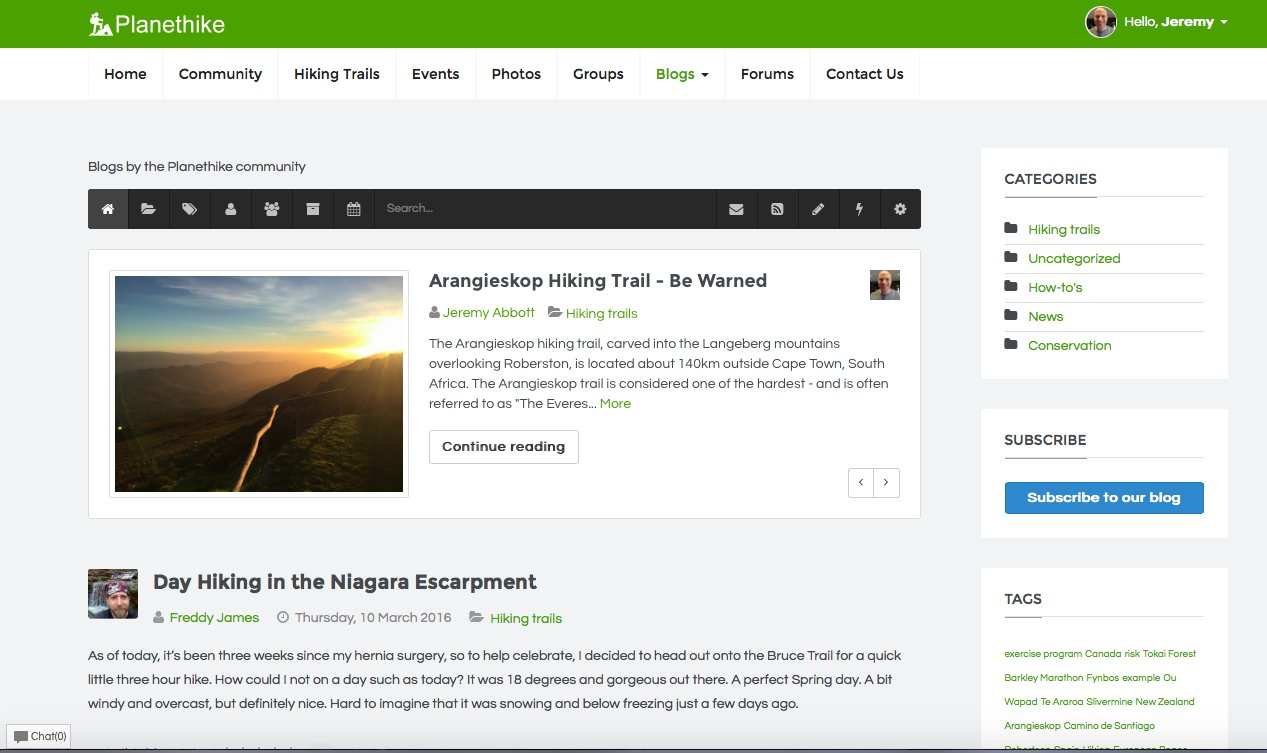
\includegraphics[width=320pt]{slike/planethike1.JPG}}
\hspace{10 pt}
\subfigure[]{\label{fig:b}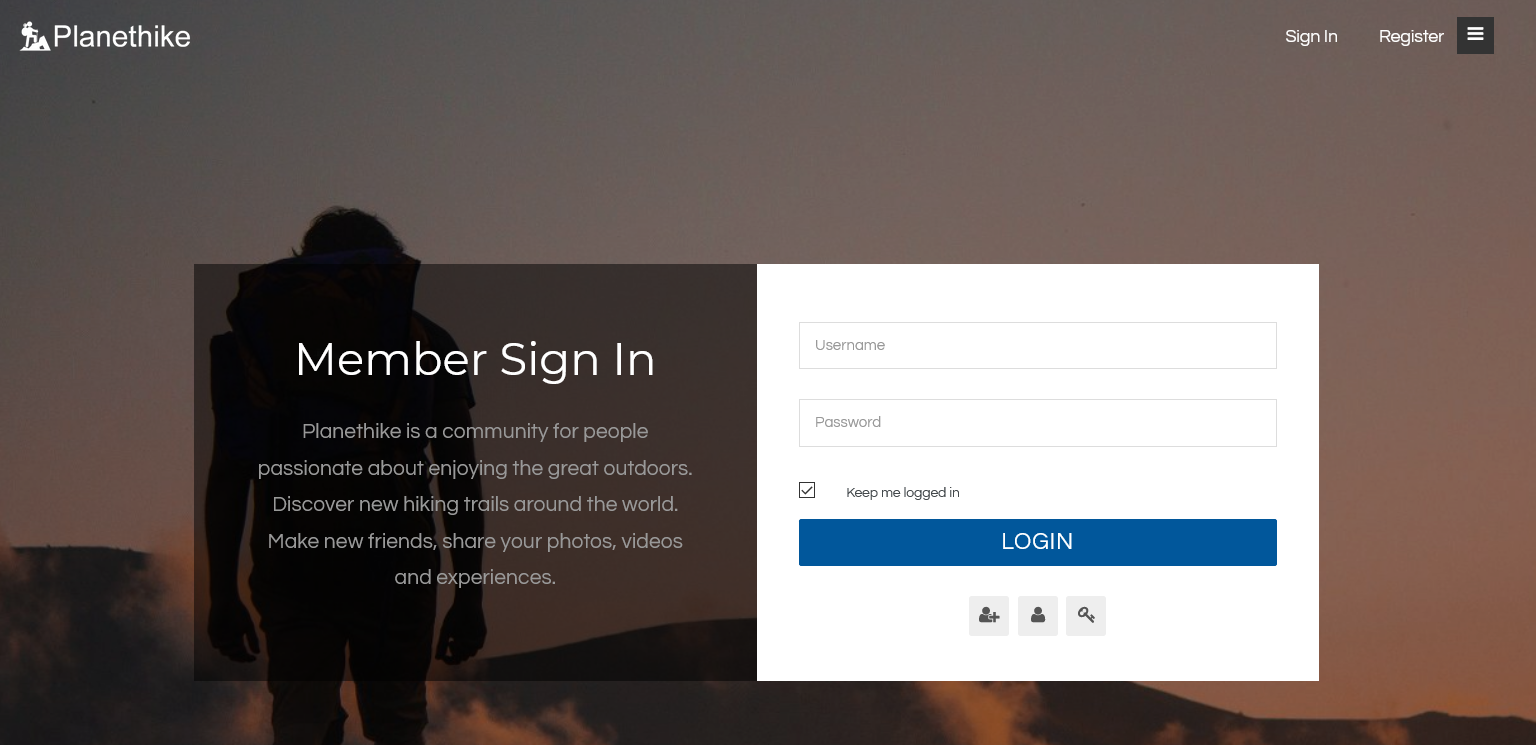
\includegraphics[width=320pt]{slike/planethike2.JPG}}
\hspace{10 pt}
\subfigure[]{\label{fig:c}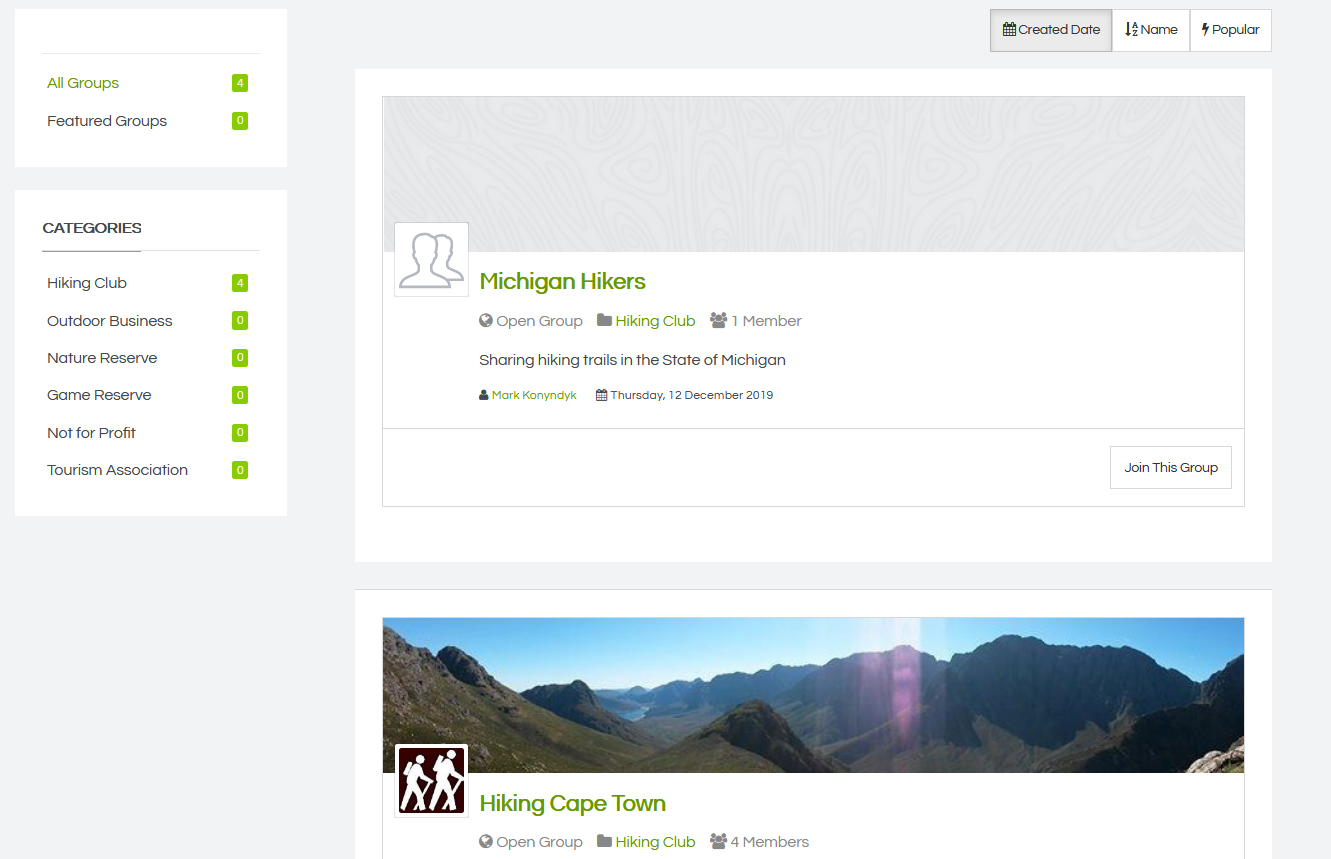
\includegraphics[width=320pt]{slike/planethike3.JPG}}
\caption{Planet hike društvena mreža}
\end{figure}

Potencijalni korisnici ove aplikacije su gotovo svi koji žele planinariti, a pritom se pripremiti za izlet ili podijeliti iskustvo nakon izleta s drugim planinarima. Pristup aplikaciji imaju svi, a korisniku se na izbor daje želi li se registrirati i prijaviti kao registrirani korisnik (hiker) ili želi samo pregledavati aplikaciju bez dodavanja sadržaja kao gost.\vspace{10pt}

\textbf{Gostu} je omogućen pregled i pretraga unaprijed definiranih planinarskih izleta koji su javni, a organizirani su prema geografskom području, trajanju i zahtjevnosti planinarskog izleta. Svaki izlet sadrži informacije o postojanju planinarskih domova i odmorišta s dostupnom infrastrukturom (prenoćište, hrana, pitka voda, struja i dr.) unutar Republike Hrvatske. \vspace{10pt}

Da bi pristupio svim funkcionalnostima aplikacije korisnik se mora registrirati i prijaviti u sustav. Podaci koje korisnik treba unijeti prilikom registracije su:

\begin{packed_item}
			\item \textit{ime}
			\item \textit{prezime}
			\item \textit{korisničko ime}
			\item \textit{lozinka}
			\item \textit{korisnička fotografija}
\end{packed_item}

Nakon uspješne registracije korisnik se nalazi na naslovnoj stranici Planinarskog dnevnika i pregledava vidljivi sadržaj na njoj; slike, događaje, bedževe i izlete. Da bi sadržaj naslovnice bio ispunjen sadržajem korisnik bi trebao dodati prijatelje čiji će se sadržaj pojavljivati. Ostale korisnike moguće je pronaći unosom određenih podataka u tražilicu na kartici \textbf{zajednica}. Kada korisnik uspostavi prijateljstva te kada njegovi prijatelju počnu objavljivati sadržaj on će, radi lakše snalažljivosti, moći filtrirati sadržaj koji mu se prikazuje na naslovnoj stranici. Sadržaj se filtrira prema sljedećim opcijama: 

\begin{packed_item}
			\item \textit {slike}
			\item \textit{događaji}
			\item \textit {bedževi}
			\item \textit{izleti}
\end{packed_item}

\textbf{Registrirani i prijavljeni korisnici} mogu kreirati vlastiti planinarski izlet (javno ili privatno) prema definiranom predlošku koji zahtijeva neke osnovne informacije:

\begin{packed_item}
			\item \textit {odredište}
			\item \textit{planinarski domovi i odmorišta}
			\item \textit{zahtjevnost izleta}
			\item \textit{dužina staze}
			\item \textit{prosječno trajanje izleta}
			\item \textit{opis izleta}
\end{packed_item} 

Pored kreiranja vlastitog planinarskog izleta, registrirani i prijavljeni korisnici mogu ocijeniti planinarski izlet te prijaviti netočne informacije, a prijavu će pregledati \textbf{administrator} ili \textbf{kreator izleta}. Ukoliko korisnik naiđe na izlet koji bi ga mogao zanimati može ga dodati na \textbf{listu željenih izleta} označavanjem ikone pored javnog izleta.
Nakon što korisnik odradi jedan od objavljenih izleta, može zatražiti potvrdu od \textbf{dežurnog planinara}. \vspace{10pt}

Nakon odrađenog niza planinarskih izleta ili stečenog postignuća korisnik može dobiti jedan ili više mogućih \textbf{bedževa} koji su implementirani kao sistem nagrađivanja. Nakon ispunjenog cilja korisnik dobije obavijest da je osvojio bedž te mu se nudi mogućnost da bedž podijeli na svom profilu i naslovnici sa svojim prijateljima. 
\vspace{10pt}

Kako bi se korisnici mogli zajedno sastati na nekom događaju ili izletu omogućena je i funkcija za kreiranje događaja. Korisnik mora biti registriran i prijavljen te odabrati karticu za \textbf{kreiranje događaja}. Važno je da u trenutku kreiranja događaja korisnik ima prijatelje koje bi mogao pozvati na događaj, u suprotnom aplikacija ne dopušta kreiranje događaja. Nakon toga ispunjava predložak koji zahtijeva neke informacije o događaju:

\begin{packed_item}
			\item \textit {naziv }
			\item \textit{datum}
			\item \textit{opis}
			\item \textit{popis pozvanih prijatelja}
\end{packed_item} 

S druge strane, korisnici koji su pozvani na događaj dobivaju prikladnu obavijesti i imaju mogućnost prihvaćanja ili odbijanja poziva. Pozivatelj nakon odgovora dobije obavijest o tome je li pozivnica prihvaćena ili odbijena.